\section{Tutorial}

\begin{frame}
  \tableofcontents[currentsection] 
\end{frame}


\begin{frame}[fragile]

\centerline{\bf Example -- Pendulum}

\begin{minipage}{0.35\textwidth}
    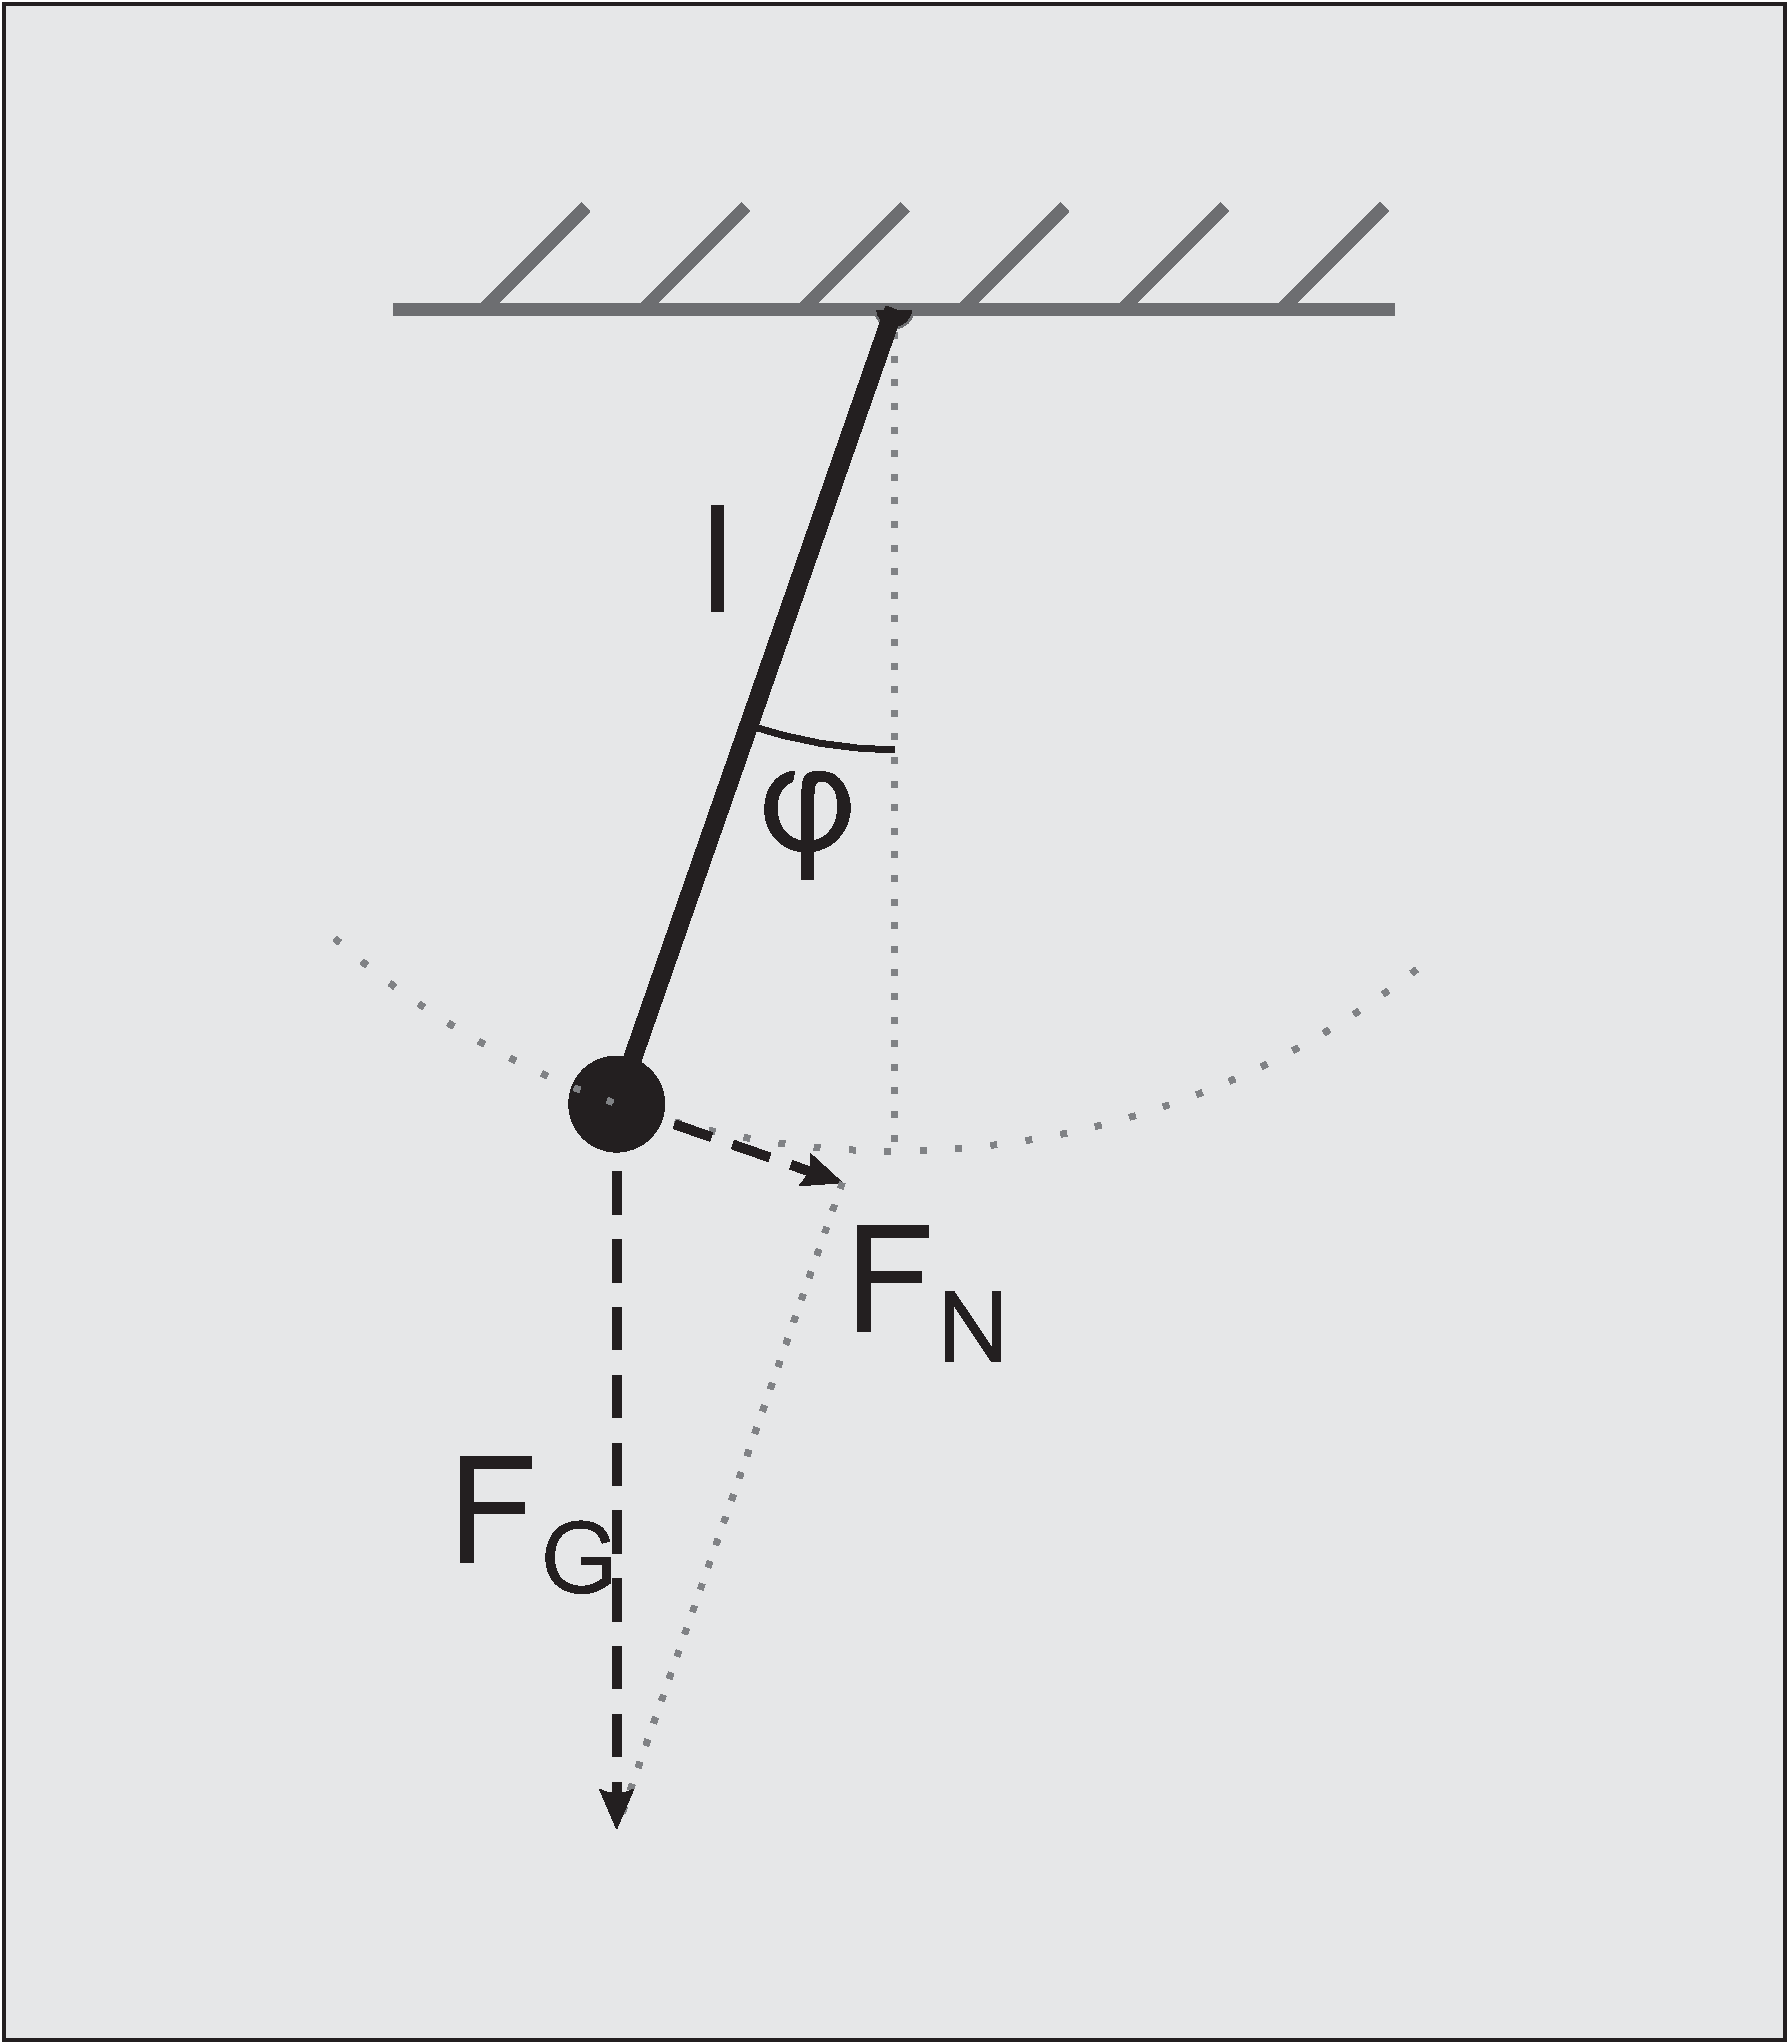
\includegraphics[draft=false,width=1.0\textwidth]{pendulum.pdf}
\end{minipage}
\hspace{2ex}
\begin{minipage}{0.5\textwidth}
 \only<1>{
 Pendulum -- Newtons law

 
 $m a = F$

 Acceleration

 $a = l \ddot{\varphi}$

 Force

 $F=F_N = - m g \sin \varphi$

 Result in an ode for the angle

 $\ddot{\varphi} = - g / l \sin \varphi $
 }

 \only<2>
 {

 $\ddot{\varphi} = - g / l \sin \varphi $

 Small angle $\sin \varphi \approx \phi$

 Harmonic oscillator

 $\ddot{\varphi} = - g / l \varphi$

 An analytic solution is known

 $\varphi = A \cos \omega t + B \sin \omega t$

 Amplitude $A$ and $B$ must be determined from initial conditions:

 $\varphi(t=0) = \varphi_0$, $\dot{\varphi}(t=0) = \dot{\varphi}_0$

 $B=\varphi_0$, $A=\dot{\varphi}_0 / \omega$

 }

 \only<3>{

 Full equation $\ddot{\varphi} = g / l \sin \varphi $

 has also analytic solution Jacobi elliptic function

 Lets enhance the ODE, add friction and external driving

 $\ddot{\varphi} = g / l \sin \varphi - \mu \dot{\varphi} + \varepsilon \sin \omega t $

 No analytic solution is known. We need to solve this equation numerically.

 }

 \only<4>{

 $\ddot{\varphi} = g / l \sin \varphi - \mu \dot{\varphi} + \varepsilon \sin \omega t $

 Create a first order ODE

 $x_1 = \varphi$, $x_2 = \dot{\varphi}$

 $\dot{x_1} = x_2$, $\dot{x_2} = - g / l \sin x_1 - \mu x_2 + \varepsilon \sin \omega t$

 $x_1$ and $x_2$ are the state space variables.

 }
 
\end{minipage}

 
\end{frame}


\begin{frame}[fragile]

\centerline{ \Large Let's solve the pendulum example numerically}
$\dot{x_1} = x_2$, $\dot{x_2} = - g / l \sin x_1 - \mu x_2 + \varepsilon \sin \omega t$

\begin{lstlisting}
#include <boost/numeric/odeint.hpp>

namespace odeint = boost::numeric::odeint;
\end{lstlisting}

\begin{lstlisting}
typedef std::array< double , 2 > state_type;
\end{lstlisting}

\begin{lstlisting}
struct pendulum
{
  double m_mu , m_omega , m_epsilon;

  pendulum( double mu , double omega , double epsilon )
  : m_mu( mu ) , m_omega( omega ) , m_epsilon( epsilon ) { }

  void operator()( const state_type &x , state_type &dxdt , double t ) const
  {
    dxdt[0] = x[1];
    dxdt[1] = - sin( x[0] ) - m_mu * x[1] + m_epsilon * sin( m_omega * t );
  }
};
\end{lstlisting}

\end{frame}

\begin{frame}[fragile]
 \centerline{ \Large Let's solve the pendulum example numerically}

$\varphi(0) = 1$, $\dot{\varphi}(0) = 0$

\begin{lstlisting}
odeint::euler< state_type > euler;
pendulum p( 0.1 , 1.05 , 1.5 );

state_type x = {{ 1.0 , 0.0 }};
double t = 0.0;

const double dt = 0.01;
euler.do_step( p , x , t , dt );
t += dt;
\end{lstlisting}

$x(0) \mapsto x(\Delta t)$

\begin{lstlisting}
std::cout << t << " " << x[0] << " " << x[1] << "\n";
for( size_t i=0 ; i<10 ; ++i )
{
  euler.do_step( p , x , t , dt );
  t += dt;
  std::cout << t << " " << x[0] << " " << x[1] << "\n";
}
\end{lstlisting}

$x(0) \mapsto x(\Delta t) \mapsto x(2\Delta t) \mapsto x(3\Delta) \mapsto \dots$

\end{frame}


\begin{frame}[fragile]
 Simulation

 $\mu=0$, $\omega_E = 0$, $\varepsilon=0$

 $\mu=0.1$, $\omega_E = 0$, $\varepsilon=0$

 $\mu=0.1$, $\omega_E = 1.05$, $\varepsilon=1.5$
\end{frame}


\begin{frame}[fragile]
 integrate functions
\end{frame}

\begin{frame}[fragile]
 steppers, rk4, rk78
\end{frame}

\begin{frame}[fragile]
 controlled steppers
\end{frame}

\begin{frame}[fragile]
 dense output stepper
\end{frame}



